% !TEX program = lualatex
% 東京電力エリア 1時間電力需要「2日後予測」レポート
% ビルド方法: リポジトリ直下で `make report` (latexmk -lualatex)
% 注意: 日本語クラス ltjsarticle を使うため LuaLaTeX 専用(pdflatexでは通らない)
\documentclass[a4paper,11pt]{ltjsarticle}

\usepackage{amsmath}
\usepackage{bm}
\usepackage{graphicx}
\usepackage{booktabs}
\usepackage[hidelinks]{hyperref}
\usepackage{xurl}

\emergencystretch=3em

\graphicspath{{assets/}}

\title{東京電力エリア 1時間電力需要「2日後予測」レポート}
\author{玉腰勇司 \\ 情報理工学系研究科数理情報学専攻修士2年 \\ 学籍番号: 48256223}
\date{\today}

\begin{document}
\maketitle

\section*{概要}

東京電力エリアの1時間電力需要 $y_t$（万kW）に対し、\textbf{2日
後（25〜48時間先）を予測するモデル}を構築し、直近1週間で検証した。
データは2016-04-01〜2026-03-31の10年分（87,648時間、
欠損なし、平均3,228万kW）である。

本レポートでは、%
\textbf{ARMA}（364日差分）と\textbf{状態空間モデル}（カ
ルマンフィルタ）の2つを基本モデルとして実装し、
応用として\textbf{ARMAX}（外生変数の追加）と\textbf{平均パ
ターン＋残差ARIMA}（周期成分の置き換え）を検討する。
流れは次の通り。

\begin{enumerate}
  \item \textbf{基本モデル}：年周期を364日差分で取り除いて定常化
  した系列への\textbf{ARMA}と、
  レベル＋日・週周期を観測方程式・システム方程式で記述しカルマンフィルタで推定す
  る\textbf{状態空間モデル}（MAPE 7.2\%）を実装する。
  \item \textbf{検証}：ARMAの2日後予測が\textbf{「前年
  値 $y_{t-364\text{日}}$ とほぼ同じ」}になることをデータで示
  す（相関0.999、
  平均差は需要の1.2\%）。
  定常系列の予測は数時間で平均に減衰するため、2日先ではARMAの補正がほぼ消える
  ことが原因である。
  \item \textbf{応用}：外生変数（雨・祝日）を加えた\textbf{ARMAX}と、
  周期成分を「前年の1観測」から\textbf{年・週・日周期の平均パターン}に置
  き換えた\textbf{平均パターン＋残差ARIMA}を検討する。%
  ARMAXは精度を改善しない一方、
  平均パターン＋残
  差ARIMAはMAPEを14.6\% $\rightarrow$ \textbf{6.2\%}に
  半減させ、
  全モデル中最良となる。
\end{enumerate}

\section{背景：日本の電力市場と「2日後」予測}

日本の電力市場で取引される電力は、市場によって受渡時期が異なる。
中心となるのは、JEPXの一日前市場（スポット市場）と当日市場（時間前市場）である。%
JEPXは、主要市場として一日前市場を、その後の調整市場として当日市場を開設して
いる\cite{jepx}。

一日前市場（スポット市場）では、翌日に受け渡される電気を取引する。%
1日を30分単位に区切った48商品として取引されるため、
例えば「翌日13:00--13:30の電力」「翌日13:30--14:00の電
力」のように、翌日の各30分コマの電力を売買する市場である。%
JEPXの説明でも、スポット市場は「翌日に受渡する電気」の市場であり、1日
を30分単位に区切った48商品を取引するとされている\cite{jepx}。

スポット市場の後には、当日市場（時間前市場）がある。
これは、スポット市場で翌日分の取引が行われた後、実際の受渡までの間に発電不調や需
要増加などが起きた場合に、需給ミスマッチを修正するための市場である。%
JEPXは、時間前市場を「翌日計画策定後の不測の需給ミスマッチに対応するための市
場」と説明している\cite{jepx}。

時間前市場では、0:00--24:00を30分単位で分割した48商品をザラバ取引する。
取引は毎日17:00に、翌日0:00--24:00の48商品について開始され、各
時間帯の受渡時間の1時間前まで取引可能である\cite{meti}。
したがって、例えば「明日13:00--13:30の電力」は前日17:00以降に時
間前市場で売買でき、受渡の1時間前まで調整できる。

先渡市場では、将来時点に受け渡される電力を取引する。
制度上は、スポット市場・時間前市場より前の段階で、将来の電力価格や調達量をヘッジ
・確保する目的で使われる。
経済産業省資料では、電力取引の流れとして、先渡市場が実需給の3年前--3日前、ス
ポット市場が前日、
時間前市場が前日17時以降から当日1時間前まで、という位置づけで示されてい
る\cite{meti}。

また、TOCOM/JPXの電力先物は、実物の電力そのものを受け渡す市場ではなく、%
JEPXスポット市場価格を参照する現金決済の先物取引である。
例えば月間物のベースロード電力は、JEPXスポット市場の東京・関西・中部エリアの
ベースロード、すなわち0:00--24:00価格を標準品としている。
日中ロード電力は8:00--20:00価格を標準品としている\cite{jpx}。

\begin{table}[htbp]
  \centering
  \caption{日本の電力市場における取引対象}
  \small
  \begin{tabular}{p{0.24\linewidth}p{0.27\linewidth}p{0.13\linewidth}p{0.24\linewidth}}
    \toprule
    市場 & 取引している電力 & 時間単位 & 主な目的 \\
    \midrule
    一日前市場（スポット市場） & 翌日に受渡する電力 & 30分$\times$48コマ & 翌日分の基本的な売買 \\
    当日市場（時間前市場） & 翌日--当日の受渡直前の電力 & 30分$\times$48コマ & 予測誤差・発電不調・需要変動の調整 \\
    先渡市場 & 数日前--数年先など将来期間の電力 & 商品設計による & 価格変動リスクのヘッジ、将来調達 \\
    電力先物 & JEPXスポット価格を参照する現金決済商品 & 月間物など & 価格リスクのヘッジ \\
    \bottomrule
  \end{tabular}
\end{table}

したがって、発電量予測や需要予測との関係で特に重要なのは、\textbf{前日段
階で翌日の48コマを予測すること}と、
実需給の数時間前に時間前市場向けに予測を更新することである。
本レポートで「2日後（25〜48時間先）」を予測対象とするのは、スポット市場で翌
日分を入札する前日段階に対応させるためである。
すなわち、翌日終日の需要を見通す状況を想定している。

\section{データと検証設計}

\begin{table}[htbp]
  \centering
  \caption{データと検証の設定}
  \begin{tabular}{lp{0.72\linewidth}}
    \toprule
    項目 & 設定 \\
    \midrule
    データ期間 & 2016-04-01 〜 2026-03-31（87,648時間） \\
    テスト週 & 2026-03-25 〜 2026-03-31（168時間） \\
    予測ホライズン & 2日後（各予測起点から25〜48時間先） \\
    検証方式 & 日単位ローリング：各テスト日 $D$ の需要を $D-2$ 日の23:00までのデータから再帰的に予測（起点を1日ずつずらして7回） \\
    評価指標 & RMSE・MAE・MAPE(\%)（168時間すべてが「2日後予測」） \\
    ARMA学習窓 & 予測起点直前の2年間 \\
    \bottomrule
  \end{tabular}
\end{table}

需要データは東京電力パワーグリッドが公開する電力使用実績\cite{tepco}を用いた。
後述のARMAXで使う雨ダミーはOpen-Meteoの東京の時別気象デー
タ\cite{openmeteo}、
祝日ダミーは内閣府の祝日一覧\cite{cao}から作成した。

「1週間先をまとめて予測」する従来構成と異なり、テスト週の\textbf{すべて
の時点が25〜48時間先の予測}として評価される点が本レポートの特徴である。

予測対象を定式化すると、各テスト日 $D$ について、$D-2$ 日
の23:00を予測起点 $t$ として
\begin{equation*}
  \hat{y}_{t+h\mid t}, \qquad h = 25, \dots, 48,
\end{equation*}
すなわち当日 $D$ の24時間分の需要を再帰的に予測する。
予測の再帰は途中の $D-1$ 日分（$h=1,\dots,24$）も通るが、評価には使わない。
この手続きを起点を1日ずつずらして7回繰り返す（図\ref{fig:scheme}）。
以降の各モデルで、この $\hat{y}_{t+h\mid t}$ の具体形を示す。

\begin{figure}[htbp]
  \centering
  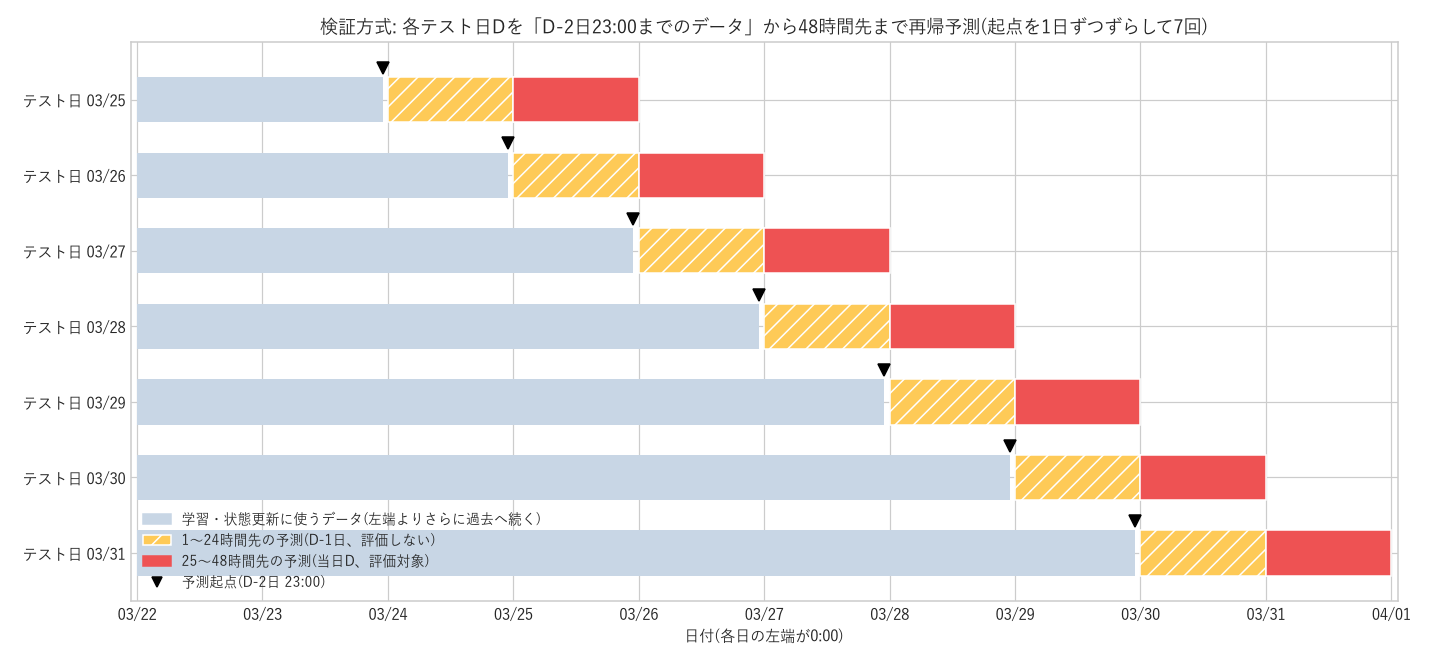
\includegraphics[width=\linewidth]{fig_2day_scheme.png}
  \caption{検証方式の模式図。
  各テスト日 $D$ を「$D-2$日23:00までのデータ」（青）から48時間先
  まで再帰予測し、%
  $D-1$日分（黄）は捨てて当日 $D$ 分（赤）のみ評価する。
  起点（▼）を1日ずつずらして7回繰り返す。%
  }
  \label{fig:scheme}
\end{figure}

\section{基本モデル}

基本モデルとして、364日差分で定常化した系列に当て
る\textbf{ARMA}と、カルマンフィルタで推定する\textbf{状態空
間モデル}の2つを実装する。

\subsection{定常性の確認（ADF検定）}

まず元系列と、年周期を取り除いた364日差分系列の推移を
図\ref{fig:series}に示す。
元系列には夏（冷房）と冬（暖房）に高く春秋に低い年周期がはっきり現れる。%
364日差分 $z_t = y_t - y_{t-8736}$ を取るとこの年周
期（および日・週周期）が消え、平均ほぼ0の変動だけが残る。

\begin{figure}[htbp]
  \centering
  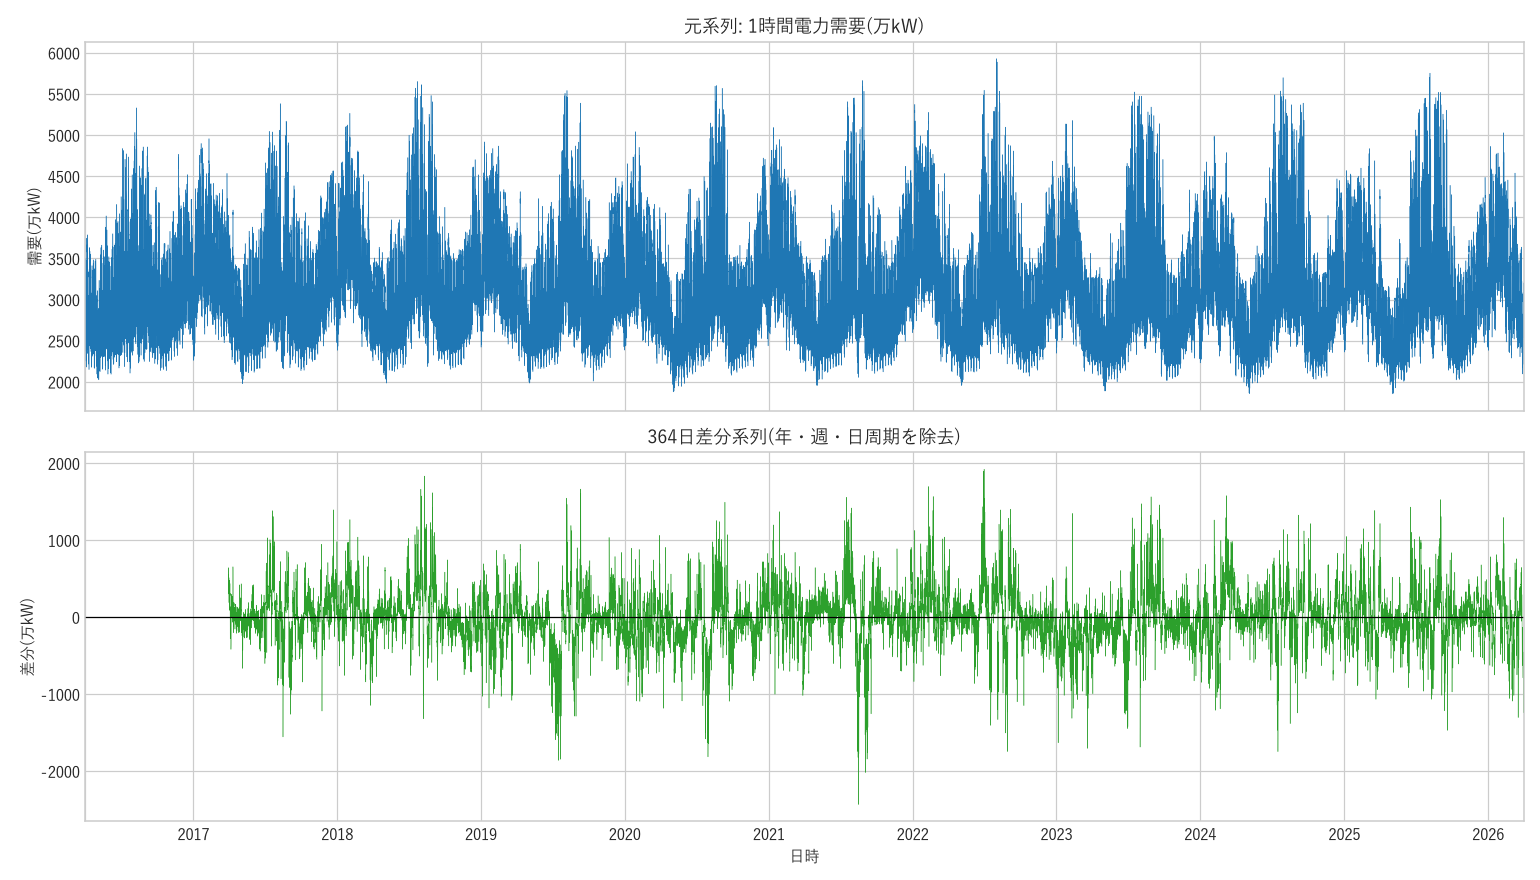
\includegraphics[width=\linewidth]{fig_2day_series.png}
  \caption{元系列（上）と364日差分系列（下）の推移}
  \label{fig:series}
\end{figure}

\begin{table}[htbp]
  \centering
  \caption{ADF検定の結果}
  \begin{tabular}{lrrrl}
    \toprule
    系列 & ADF統計量 & p値 & 分散 & 5\%で定常? \\
    \midrule
    元系列 & $-20.88$ & 0.000 & 459,342 & Yes \\
    1次差分 & $-48.13$ & 0.000 & 26,770 & Yes \\
    24時間差分 & $-38.45$ & 0.000 & 99,535 & Yes \\
    168時間差分 & $-24.31$ & 0.000 & 146,174 & Yes \\
    \textbf{364日差分} & $\mathbf{-21.90}$ & \textbf{0.000} & \textbf{123,904} & \textbf{Yes} \\
    \bottomrule
  \end{tabular}
\end{table}

元系列も形式的にはADF検定を通るが、ACFにはラグ24（0.892）・ラ
グ168（0.840）の強い周期相関が残る。%
24時間差分は日周期を、168時間差分は日・週周期を取り除けるが、いずれも年周期は残る。%
364日差分 $z_t = y_t - y_{t-8736}$ は「昨年の同じ曜
日・同じ時刻」との差を取るため、日・週・年の3つの周期を一度に取り除ける。
分散も元系列の約1/4に減り、これを定常系列とみなしてARMAを当てる。

\begin{figure}[htbp]
  \centering
  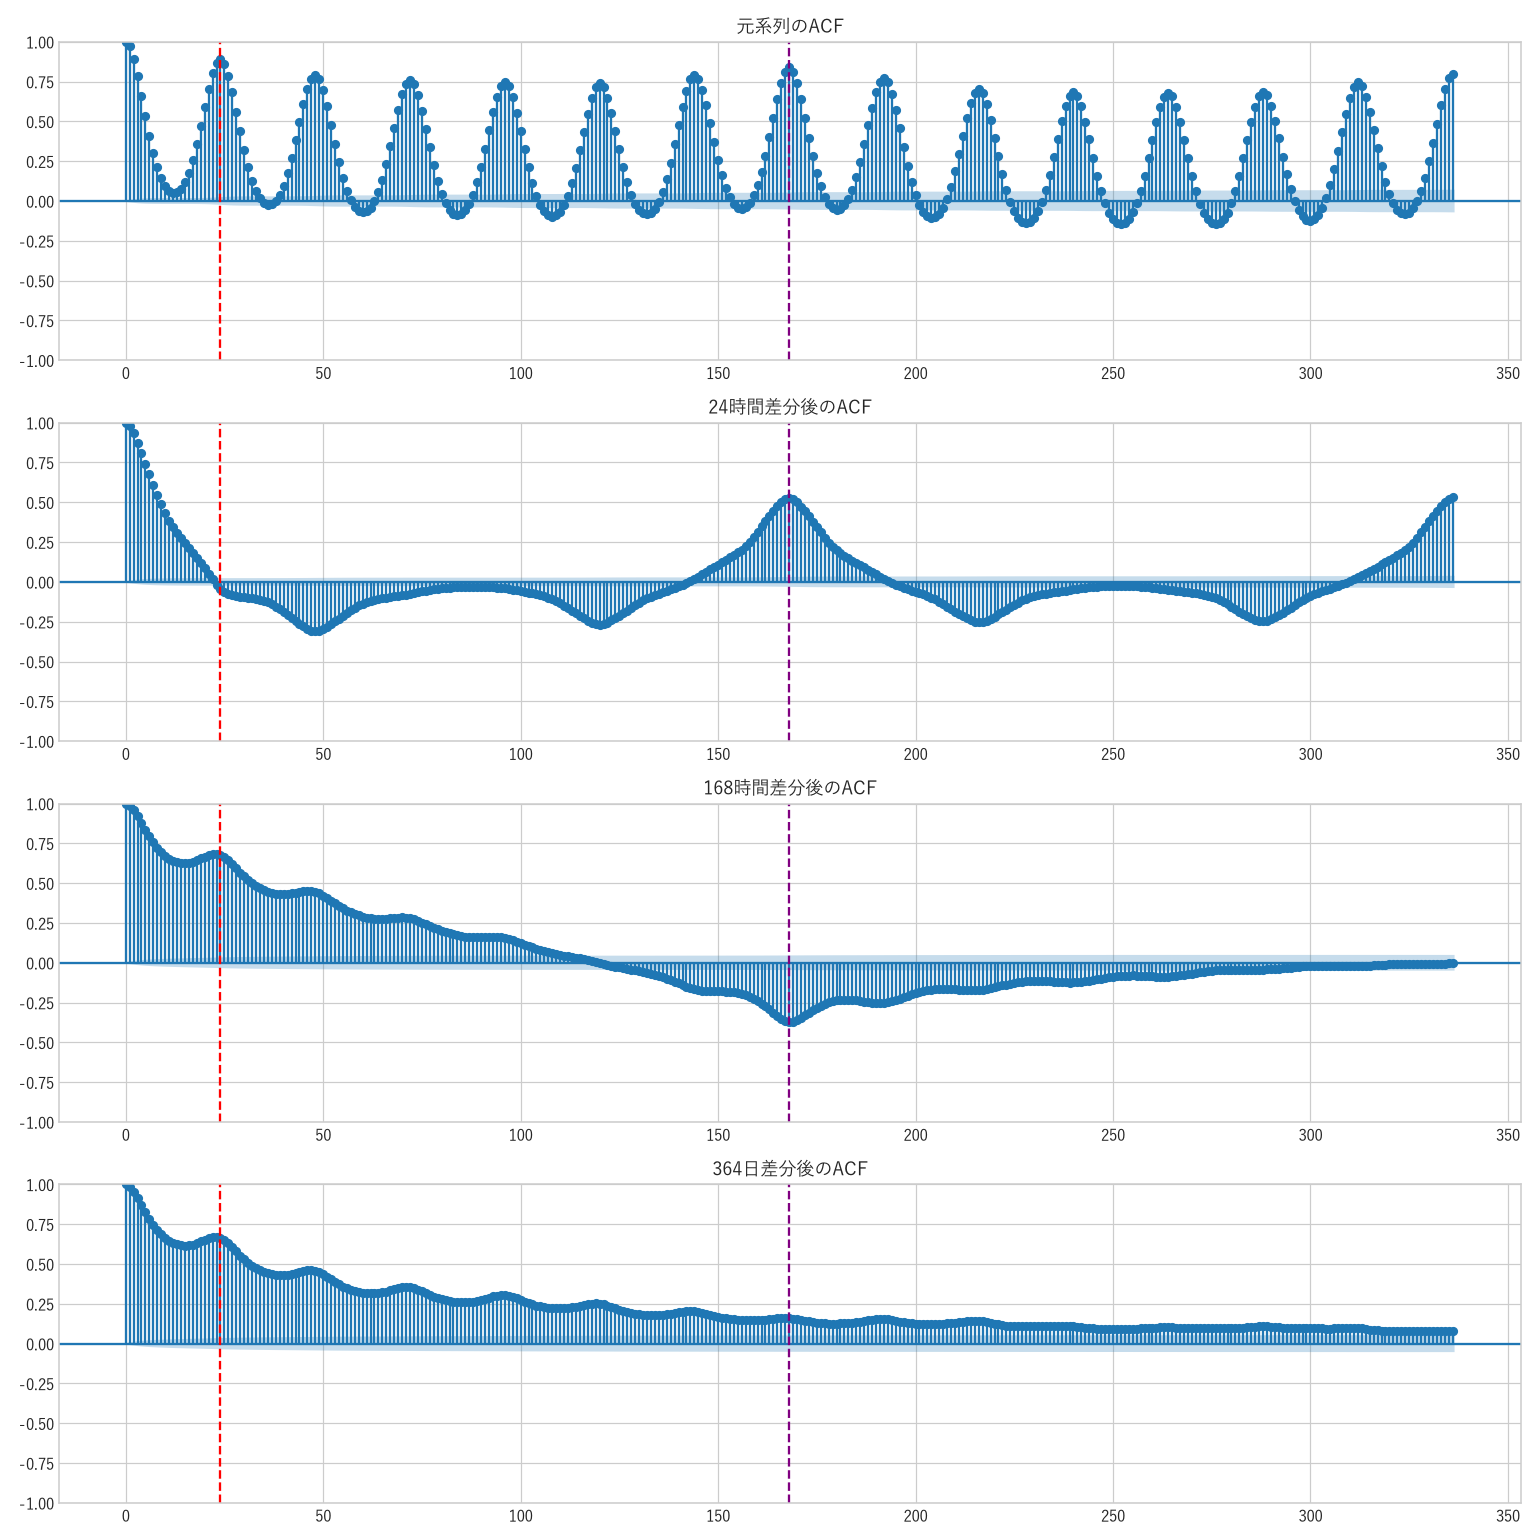
\includegraphics[width=0.92\linewidth]{fig_2day_acf.png}
  \caption{元系列と差分系列のACF}
\end{figure}

\subsection{364日差分 + ARMA}

差分系列 $z_t = y_t - y_{t-8736}$ にARMA($p,q$)モデル
\begin{equation*}
  z_t = c + \sum_{i=1}^{p} \phi_i z_{t-i} + \varepsilon_t + \sum_{j=1}^{q} \theta_j \varepsilon_{t-j},
  \qquad \varepsilon_t \sim \mathrm{i.i.d.}\ (0, \sigma^2)
\end{equation*}
を当て、\textbf{AICで次数を選択}した。参考として、各候補の2日後ロー
リング検証の精度（RMSE・MAE・MAPE）も併記する。

\begin{table}[htbp]
  \centering
  \caption{ARMAの次数選択（AIC）と参考精度}
  \begin{tabular}{lrrrr}
    \toprule
    モデル & AIC & （参考）RMSE & MAE & MAPE \\
    \midrule
    \textbf{ARMA(2,2)} & \textbf{183,646} & 496.3 & 413.8 & 14.61\% \\
    ARMA(2,1) & 183,659 & 497.3 & 415.0 & 14.65\% \\
    ARMA(2,0) & 183,815 & 502.9 & 420.7 & 14.86\% \\
    ARMA(1,1) & 185,255 & 464.1 & 379.3 & 13.41\% \\
    ARMA(1,0) & 191,778 & 447.4 & 359.4 & 12.76\% \\
    \bottomrule
  \end{tabular}
\end{table}

AICが最良だったのは\textbf{ARMA(2,2)}であり、以降これを採用
する。なおテスト精度はどの次数でも13〜15\%の狭い範囲にある。

選択されたARMA(2,2)の係数（参考、すべて364日差分系列上のもの）を
表\ref{tab:arma-coef}に示す。

\begin{table}[htbp]
  \centering
  \caption{ARMA(2,2)の係数}
  \label{tab:arma-coef}
  \begin{tabular}{lr}
    \toprule
    係数 & 推定値 \\
    \midrule
    const & 18.31 \\
    ar.L1 & 1.445 \\
    ar.L2 & $-0.476$ \\
    ma.L1 & 0.188 \\
    ma.L2 & 0.033 \\
    \bottomrule
  \end{tabular}
\end{table}

AR係数の和（$1.445-0.476 \approx 0.97$）が1に近く、
強い持続性を持つ系列であることがわかる。予測対象は、
差分系列の予測 $\hat{z}$ を前年値に足して元の水準に戻した
\begin{equation*}
  \hat{y}_{t+h\mid t} = y_{t+h-8736} + \hat{z}_{t+h\mid t}, \qquad h = 25, \dots, 48
\end{equation*}
である。

\subsection{検証：予測は「前年値」とほぼ変わらない}
\label{sec:verify}

\subsubsection{データによる確認}

テスト週168時間について、ARMA予測と前年値を直接比較した。

\begin{table}[htbp]
  \centering
  \caption{予測と前年値の近さ}
  \begin{tabular}{lrrr}
    \toprule
    モデル & 前年値との平均絶対差（万kW） & 需要比 & 前年値との相関 \\
    \midrule
    364日差分+ARMA(2,2) & 32.3 & \textbf{1.15\%} & \textbf{0.9990} \\
    \bottomrule
  \end{tabular}
\end{table}

補正量は最大でも63万kW（需要の約2\%）で、予測精度もほぼ同じである。

\begin{table}[htbp]
  \centering
  \caption{予測精度の比較（前年値との対比）}
  \begin{tabular}{lrrr}
    \toprule
    モデル & RMSE & MAE & MAPE \\
    \midrule
    364日差分+ARMA(2,2) & 496.3 & 413.8 & 14.61\% \\
    （参考）前年値をそのまま使った場合 & 503.9 & 425.5 & 15.00\% \\
    \bottomrule
  \end{tabular}
\end{table}

\begin{figure}[htbp]
  \centering
  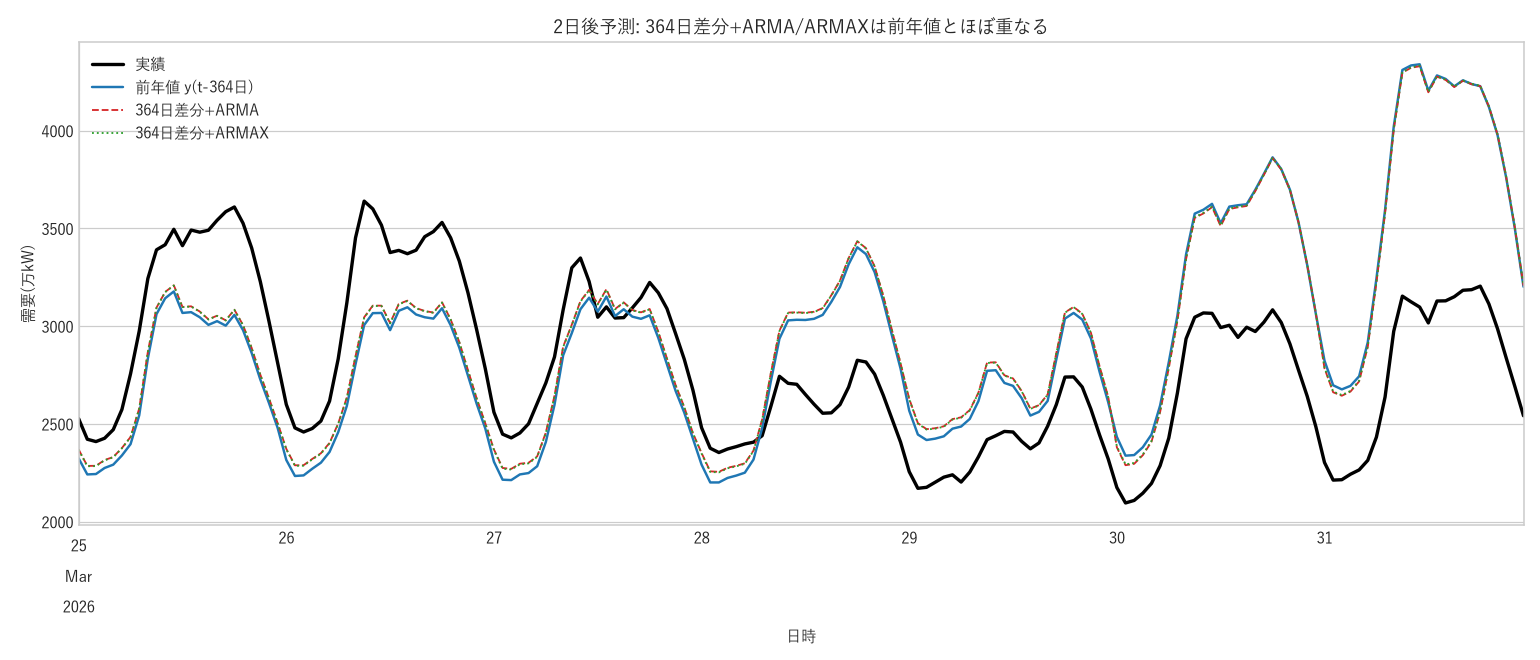
\includegraphics[width=\linewidth]{fig_2day_arma_vs_lastyear.png}
  \caption{ARMA予測と前年値の比較}
\end{figure}

ARMA（赤破線）は前年値（青）にほぼ重なっており、%
2日後予測としては「前年値コピー」と実質同等であることが図からも確認できる（緑の
点線は第\ref{sec:armax}節のARMAXで、
同様に前年値に重なる）。

\subsubsection{何が問題か}

問題は、「前年コピー」が前年固有のノイズも引き継いでしまう点にある。
テスト週の実績は前年より大幅に低く（気温等の年々変動）、前年値のMAPEは15\%に達する。%
\textbf{前年のたった1本の観測値}には、その年固有の天候・曜日配置のノイ
ズがそのまま乗っており、%
364日差分+ARMAはこのノイズを2日後予測でほぼ補正できない。

\subsection{状態空間モデル（カルマンフィルタ）}
\label{sec:statespace}

もう一つの基本モデルとして、需要を観測不能な状態変数（レベル・季節成分）の和で表
す\textbf{状態空間モデル}を構築し、
カルマンフィルタで推定する。モデルは観測方程式とシステム方程式で記述される。

\textbf{観測方程式}（観測値 $y_t$ と状態の関係）：
\begin{equation*}
  y_t = \mu_t + \gamma^{(24)}_t + \gamma^{(168)}_t + \varepsilon_t,
  \qquad \varepsilon_t \sim \mathrm{N}(0, \sigma^2_\varepsilon)
\end{equation*}

\textbf{システム方程式}（状態の時間発展）：レベル成
分 $\mu_t$ はランダムウォーク
\begin{equation*}
  \mu_{t+1} = \mu_t + \eta_t, \qquad \eta_t \sim \mathrm{N}(0, \sigma^2_\eta)
\end{equation*}
に従う。
周期 $s$（日周期 $s=24$、週周期 $s=168$）の季節成分は三角関数
型の確率的季節成分であり、
調波の
和 $\gamma^{(s)}_t = \sum_{j=1}^{k} \gamma_{j,t}$ と
して、各調波 $j$ が
\begin{equation*}
  \begin{pmatrix} \gamma_{j,t+1} \\ \gamma^{*}_{j,t+1} \end{pmatrix}
  =
  \begin{pmatrix} \cos\lambda_j & \sin\lambda_j \\ -\sin\lambda_j & \cos\lambda_j \end{pmatrix}
  \begin{pmatrix} \gamma_{j,t} \\ \gamma^{*}_{j,t} \end{pmatrix}
  +
  \begin{pmatrix} \omega_{j,t} \\ \omega^{*}_{j,t} \end{pmatrix},
  \qquad \lambda_j = \frac{2\pi j}{s}
\end{equation*}
と時間発展する（日周期は $k=8$、週周期は $k=6$ 調波）。

状態はカルマンフィルタで観測値から逐次推定し、分散パラメータは最尤法で推定した（
学習窓は他モデルと同じ直近2年）。予測対象は、
予測起点 $t$ までフィルタリングした状態の $h$ ステップ先予測
\begin{equation*}
  \hat{y}_{t+h\mid t} = \hat{\mu}_{t+h\mid t} + \hat{\gamma}^{(24)}_{t+h\mid t} + \hat{\gamma}^{(168)}_{t+h\mid t},
  \qquad h = 25, \dots, 48
\end{equation*}
であり、他モデルと同じ日単位ローリング方式で検証した。

\begin{table}[htbp]
  \centering
  \caption{状態空間モデルの分散パラメータ}
  \begin{tabular}{lr}
    \toprule
    分散パラメータ & 推定値 \\
    \midrule
    $\sigma^2$（観測ノイズ） & $\approx 0$ \\
    $\sigma^2$（レベル） & 356.0 \\
    $\sigma^2$（日周期） & 0.69 \\
    $\sigma^2$（週周期） & 323.0 \\
    \bottomrule
  \end{tabular}
\end{table}

レベルと週周期の分散が大きく推定されており、水準と週の形が時間とともに大きく動く
系列であることをモデル自身が捉えている。

\begin{table}[htbp]
  \centering
  \caption{状態空間モデルの予測精度}
  \begin{tabular}{lrrr}
    \toprule
    モデル & RMSE & MAE & MAPE \\
    \midrule
    状態空間モデル（カルマンフィルタ） & 230.0 & 196.4 & \textbf{7.19\%} \\
    （参考）364日差分+ARMA(2,2) & 496.3 & 413.8 & 14.61\% \\
    \bottomrule
  \end{tabular}
\end{table}

MAPEは7.19\%であり、%
ARMA（14.6\%）より大幅に低い。ランダムウォークのレベ
ル $\mu_t$ が直近の水準ずれに自動的に追随し、
予測が「前年値コピー」に縛られないためである。

\section{応用}

基本モデルを踏まえ、2つの拡張を検討する。外生変数を加える\textbf{ARMAX}と、
周期成分の表し方を置き換える\textbf{平均パターン＋残差ARIMA}である。

\subsection{ARMAX：外生変数の追加（雨・祝日）}
\label{sec:armax}

同じ差分系列に、%
364日差分した外生変数 $\bm{x}_t$（$\Delta$雨ダミー
・$\Delta$祝日ダミー）の回帰項を加えたARMAX($p,q$)モデル
\begin{equation*}
  z_t = c + \bm{\beta}^\top \bm{x}_t + \sum_{i=1}^{p} \phi_i z_{t-i} + \varepsilon_t + \sum_{j=1}^{q} \theta_j \varepsilon_{t-j}
\end{equation*}
を推定し、ARMAと同様に\textbf{AICで次数を選択}した。予測対象もARMAと同じく
\begin{equation*}
  \hat{y}_{t+h\mid t} = y_{t+h-8736} + \hat{z}_{t+h\mid t}, \qquad h = 25, \dots, 48
\end{equation*}
であり、$\hat{z}$ の計算には外生変数の将来値を用いる（祝日は既知。雨は
本来予報を用いるべきところ、ここでは実績値で代用した）。

\begin{table}[htbp]
  \centering
  \caption{ARMAXの次数選択（AIC）と参考精度}
  \begin{tabular}{lrrrr}
    \toprule
    モデル & AIC & （参考）RMSE & MAE & MAPE \\
    \midrule
    \textbf{ARMAX(2,1)} & \textbf{183,662} & 497.5 & 415.1 & 14.65\% \\
    ARMAX(2,0) & 183,817 & 503.1 & 420.9 & 14.86\% \\
    ARMAX(1,1) & 185,259 & 464.8 & 380.0 & 13.44\% \\
    ARMAX(2,2) & 185,351 & 496.4 & 413.8 & 14.61\% \\
    ARMAX(1,0) & 191,781 & 448.0 & 359.9 & 12.78\% \\
    \bottomrule
  \end{tabular}
\end{table}

AICが最良だったのは\textbf{ARMAX(2,1)}である。その係数と有
意性を表\ref{tab:armax-coef}に示す。

\begin{table}[htbp]
  \centering
  \caption{ARMAX(2,1)の係数と有意性}
  \label{tab:armax-coef}
  \begin{tabular}{lrrl}
    \toprule
    係数 & 推定値 & p値 & 5\%で有意? \\
    \midrule
    const & 18.47 & 0.169 & No \\
    $\Delta$雨 & $-0.16$ & 0.795 & No \\
    $\Delta$祝日 & $-3.26$ & 0.793 & No \\
    ar.L1 & 1.481 & $<0.001$ & Yes \\
    ar.L2 & $-0.511$ & $<0.001$ & Yes \\
    ma.L1 & 0.151 & $<0.001$ & Yes \\
    \bottomrule
  \end{tabular}
\end{table}

\textbf{外生変数は雨・祝日とも有意でない}。
理由としては、雨は数時間、祝日は24時間と\textbf{持続的な事象}であることが考えられる。
事象が始まって数時間も経てばその影響は直前の需要（AR項
の $z_{t-1}, z_{t-2}$）に既に現れており、
継続中の時間帯はAR項だけで十分説明できてしまう。
外生変数に固有の説明力が残るのは、事象の切り替わり（開始・終了）の時点だけである。

\subsection{平均パターン + 残差ARIMA：周期成分の置き換え}
\label{sec:profile}

第\ref{sec:verify}節で見たARMAの弱点を踏まえ、
「周期成分を取り除いてからARMA系モデルを当てる」という枠組みは同一とし、%
\textbf{周期成分の表し方だけを「前年の1観測」から「10年分の平均パター
ン」に置き換えた}モデルを構築する。

予測対象は
\begin{equation*}
  \hat{y}_{t+h\mid t} =
  \underbrace{m + d(\text{時刻}_{t+h}) + w(\text{曜日}_{t+h}, \text{時刻}_{t+h}) + a(\text{通日}_{t+h})}_{\text{平均パターン}}
  + \underbrace{\hat{r}_{t+h\mid t}}_{\text{残差のARIMA予測}}
\end{equation*}
である（$h = 25, \dots, 48$）。

\subsubsection{平均パターン（年・週・日周期の平均化）}

\begin{itemize}
  \item $m$：全体平均
  \item $d$：時刻別平均の偏差（日周期、24値）
  \item $w$：曜日$\times$時刻別平均の偏差（週周期、168値）
  \item $a$：通日別平均の偏差を31日移動平均で平滑化（年周期、366値）
\end{itemize}

\begin{figure}[htbp]
  \centering
  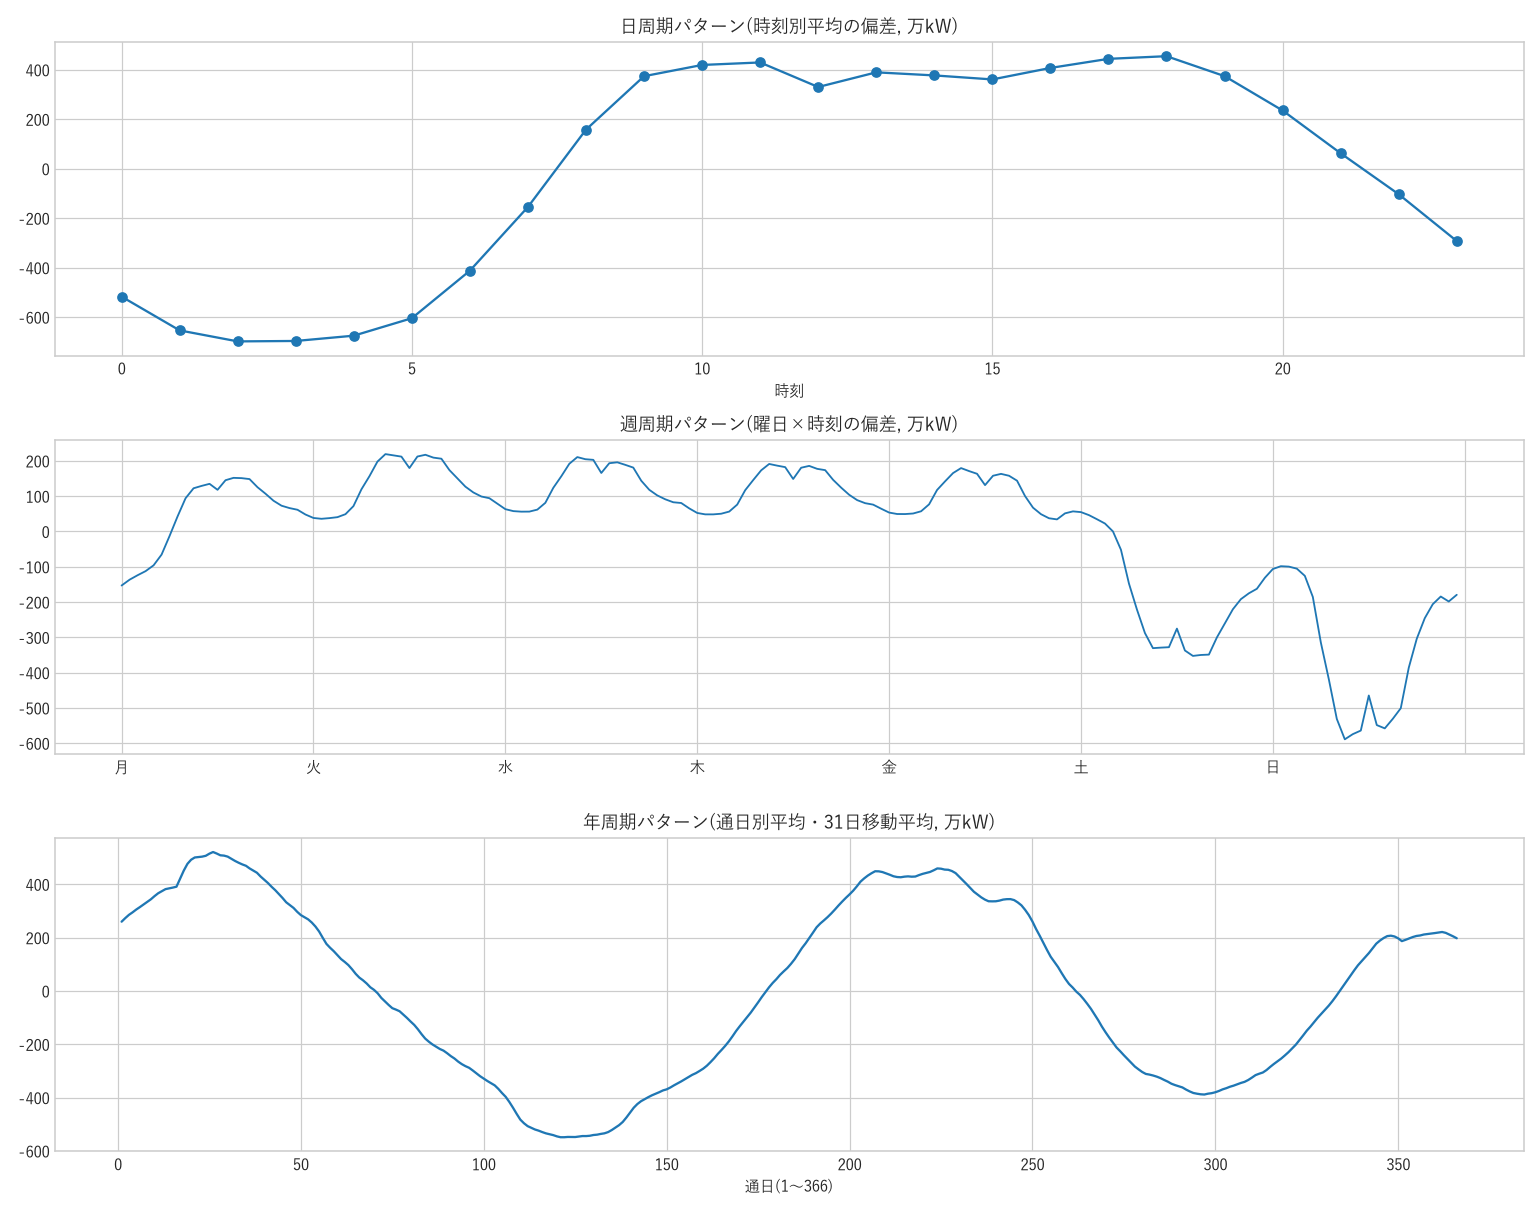
\includegraphics[width=0.92\linewidth]{fig_2day_profile.png}
  \caption{平均パターンの中身}
\end{figure}

平均化により、単年の天候ノイズは約 $1/\sqrt{10}$ に圧縮される。
周期性の除去という役割は364日差分と同じだが、「前年のノイズごとコピーする」の
ではなく「10年の平均的な形だけを反映する」点が異なる。

\subsubsection{残差のARIMA}

平均パターンを引いた残差 $r_t$ には、気温など天候起因の\textbf{持
続的な水準ずれ}が残る。
実際、残差の自己相関はラグ1で0.971、ラグ24で0.804、ラグ168で
も0.345と減衰が極めて遅い。
このような系列を定常ARMAで扱うと、予測が数時間で平均0に減衰してしまい直近の
ずれを活かせない。
そこで\textbf{1次差分を入れたARIMA($p,1,q$)}を残差に当て、直近の水準ずれを先へ引き継ぐ。
次数はAICで選択した。

\begin{table}[htbp]
  \centering
  \caption{残差モデルの次数選択（AIC）}
  \begin{tabular}{lr}
    \toprule
    残差モデル & AIC \\
    \midrule
    \textbf{ARIMA(2,1,2)} & \textbf{188,568} \\
    ARIMA(2,1,1) & 189,119 \\
    ARIMA(1,1,1) & 190,490 \\
    \bottomrule
  \end{tabular}
\end{table}

\subsubsection{検証結果}

「平均パターン + 残差ARIMA(2,1,2)」を、他モデルと同じ日単位ローリ
ング方式で検証した。

\begin{table}[htbp]
  \centering
  \caption{代替案の予測精度}
  \begin{tabular}{lrrr}
    \toprule
    モデル & RMSE & MAE & MAPE \\
    \midrule
    \textbf{平均パターン + 残差ARIMA(2,1,2)} & \textbf{200.3} & \textbf{170.0} & \textbf{6.19\%} \\
    （参考）364日差分+ARMA & 496.3 & 413.8 & 14.61\% \\
    \bottomrule
  \end{tabular}
\end{table}

誤差は年差分ARMAの半分以下になった。
改善に寄与した要因は2つある。
周期成分を平均化して\textbf{単年の天候ノイズを除去した}こと、
そして残差ARIMAの $d=1$ により2日先でも予測が0に減衰せず、%
\textbf{予測起点時点の「平年からのずれ」を保って}日 $D$ の予測に反
映できることである。

\section{総合比較}

\begin{table}[htbp]
  \centering
  \caption{全モデルの2日後予測精度（テスト週168時間）}
  \begin{tabular}{clrrr}
    \toprule
    順位 & モデル & RMSE & MAE & MAPE \\
    \midrule
    1 & \textbf{平均パターン + 残差ARIMA(2,1,2)} & \textbf{200.3} & \textbf{170.0} & \textbf{6.19\%} \\
    2 & 状態空間モデル（カルマンフィルタ） & 230.0 & 196.4 & 7.19\% \\
    3 & naive\_2day（2日前コピー） & 403.7 & 320.7 & 11.65\% \\
    4 & 364日差分+ARMA(2,2) & 496.3 & 413.8 & 14.61\% \\
    5 & 364日差分+ARMAX(2,1) & 497.5 & 415.1 & 14.65\% \\
    \bottomrule
  \end{tabular}
\end{table}

\begin{figure}[htbp]
  \centering
  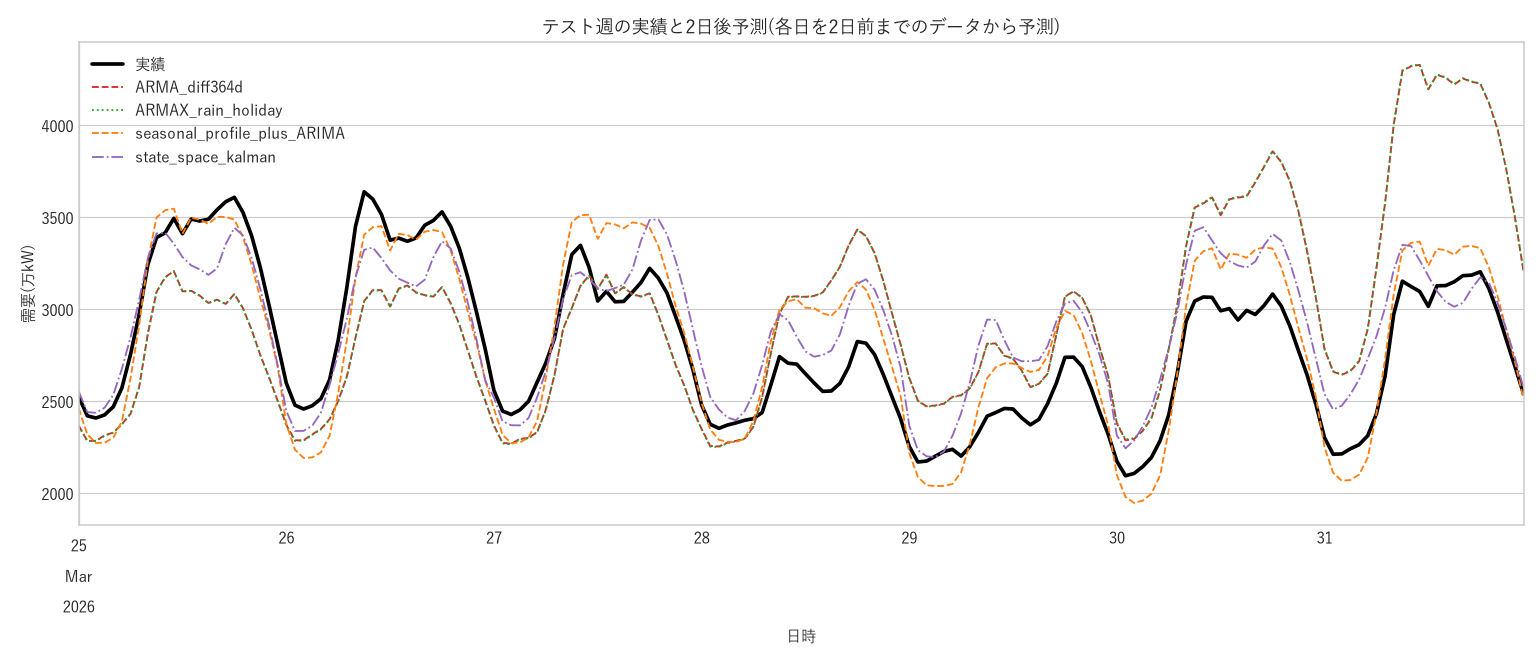
\includegraphics[width=\linewidth]{fig_2day_forecast_compare.png}
  \caption{テスト週の実績と2日後予測（各日を2日前までのデータから予測）}
\end{figure}

今回のテスト週は需要水準が平年からずれている（前年比でも低い）ため、周期構造だけ
を写す予測ではこのずれ分が誤差として残る。
「平均パターン + 残差ARIMA」は、1次差分入りの残差ARIMAが直近のずれ
を2日先まで引き継ぐことで、誤差を6.19\%に抑えている。
状態空間モデル（7.19\%）のレベル成分も同じ役割を単一のモデルの中で果たして
いるが、年周期成分を持たず、%
10年分の平均情報も使わない（直近2年の観測だけから季節形状を推定する）ぶん、
「平均パターン + 残差ARIMA」に一歩及ばなかったと考えられる。

\section{まとめ}

本レポートでは、電力需要の2日後予測のために、基本モデルとし
て\textbf{ARMA}（364日差分）と\textbf{状態空間モデル}（カルマンフィルタ）を適用し、
応用として\textbf{ARMAX}（外生変数の追加）と\textbf{周期成分の平均パターンへの置き換え}を試した。
364日差分+ARMA/ARMAXの予測は、定常モデルの補正が2日先までに減衰するた
め\textbf{前年値コピーと実質同等}だった（MAPE 14.6\%）。
状態空間モデルはMAPE 7.19\%だった。
周期成分を10年の平均パターンに置き換え、
残差に1次差分入りのARIMA(2,1,2)を当てたものが全モデル中最良
で、MAPEは\textbf{6.19\%}だった。
残る誤差の主因は2日の間の気象変化であり、%
\textbf{気温予報などの外生変数の利用}が今後の課題である。

\renewcommand{\refname}{出典}
\begin{thebibliography}{9}
  \bibitem{jepx} 日本卸電力取引所（JEPX）「取引概要」\\
    \url{https://www.jepx.jp/electricpower/outline/}
  \bibitem{meti} 経済産業省 電力・ガス取引監視等委員会 制度設計専門会合 資料\\
    \url{https://www.egc.meti.go.jp/activity/emsc_system/pdf/051_06_00.pdf}
  \bibitem{jpx} 日本取引所グループ（JPX）「電力先物」\\
    \url{https://www.jpx.co.jp/derivatives/products/energy/electricity-futures/01.html}
  \bibitem{tepco} 東京電力パワーグリッド「でんき予報」過去の電力使用実績データ\\
    \url{https://www.tepco.co.jp/forecast/html/download-j.html}
  \bibitem{openmeteo} Open-Meteo Historical Weather API（東京の時別気象データ）\\
    \url{https://open-meteo.com/}
  \bibitem{cao} 内閣府「国民の祝日について」祝日一覧CSV\\
    \url{https://www8.cao.go.jp/chosei/shukujitsu/syukujitsu.csv}
\end{thebibliography}

\section*{再現方法}

\begin{verbatim}
uv run python scripts/forecast_2day_analysis.py   # 分析の実行
make report                                       # 本レポートのコンパイル
\end{verbatim}

数値は \texttt{report/assets/results\_2day.json}、
図
は \texttt{report/assets/fig\_2day\_*.png} に
出力される。

\end{document}
